
% This LaTeX was auto-generated from an M-file by MATLAB.
% To make changes, update the M-file and republish this document.

%%% \documentclass{article}
%%% \usepackage{graphicx}
%%% \usepackage{color}

%%% \sloppy
%%% \definecolor{lightgray}{gray}{0.5}
\setlength{\parindent}{0pt}

%%% \begin{document}

    
    
\subsection*{Integral and Differential Non Linearity of ADC}

\begin{par}
Example for algorithm INL-DNL
\end{par} \vspace{1em}
\begin{par}
INL-DNL is an algorithm for estimating Integral and Differential Non-Linearity of an ADC. ADC has to sample a pure sine wave. To estimate all transition levels the amplitude of the sine wave should overdrive the full range of the ADC by at least 120\%. If not so, non estimated transition levels will be assumed to be 0 and the results may be less accurate. As an input ADC codes are required.';
\end{par} \vspace{1em}
\begin{par}
See also 'Virosztek, T., Pálfi V., Renczes B., Kollár I., Balogh L., Sárhegyi A., Márkus J., Bilau Z. T., ADCTest project site: \url{http://www.mit.bme.hu/projects/adctest} 2000-2014';
\end{par} \vspace{1em}

\subsubsection*{Contents}

\begin{itemize}
\setlength{\itemsep}{-1ex}
   \item Generate sample data
   \item Call algorithm
\end{itemize}


\subsubsection*{Generate sample data}

\begin{par}
Suppose a sine wave of nominal frequency 10 Hz and nominal amplitude 1.5 V is sampled by ADC with bit resolution of 4 and full range of 1 V. First quantity \lstinline{bitres} with number of bits of resolution of the ADC is prepared and put into input data structure \lstinline{DI}.
\end{par} \vspace{1em}
\begin{lstlisting}[style=mcode]
DI = [];
DI.bitres.v = 4;
\end{lstlisting}
\begin{par}
Waveform is constructed. Amplitude is selected to overload the ADC.
\end{par} \vspace{1em}
\begin{lstlisting}[style=mcode]
t=[0:1/1e4:1-1/1e4];
Anom = 3.5; fnom = 2; phnom = 0;
wvfrm = Anom*sin(2*pi*fnom*t + phnom);
\end{lstlisting}
\begin{par}
Next ADC code values are calculated. It is simulated by quantization and scaling of the sampled waveform. In real measurement code values can be obtained directly from the ADC. Suppose ADC range is -2..2.
\end{par} \vspace{1em}
\begin{lstlisting}[style=mcode]
codes = wvfrm;
rmin = -2; rmax = 2;
levels = 2.^DI.bitres.v - 1;
codes(codes<rmin) = rmin;
codes(codes>rmax) = rmax;
codes = round((codes-rmin)./(rmax-rmin).*levels);
\end{lstlisting}
\begin{par}
Now lets introduce ADC error. Instead of generating code 2 ADC erroneously generates code 3 and instead of 11 it generates 10.
\end{par} \vspace{1em}
\begin{lstlisting}[style=mcode]
codes(codes==2) = 3;
codes(codes==11) = 10;
codes = codes + min(codes);
\end{lstlisting}
\begin{par}
Create quantity \lstinline{codes} and plot a figure with sampled sine wave and codes.
\end{par} \vspace{1em}
\begin{lstlisting}[style=mcode]
DI.codes.v = codes;
figure
hold on
stairs(t, codes);
wvfrm = (wvfrm - rmin)./(rmax-rmin).*levels;
plot(t, wvfrm, '-r');
xlabel('t (s)')
ylabel('Codes / Voltage (scaled)');
legend('Codes generated by ADC','Original waveform scaled to match codes');
hold off
\end{lstlisting}

\begin{center}
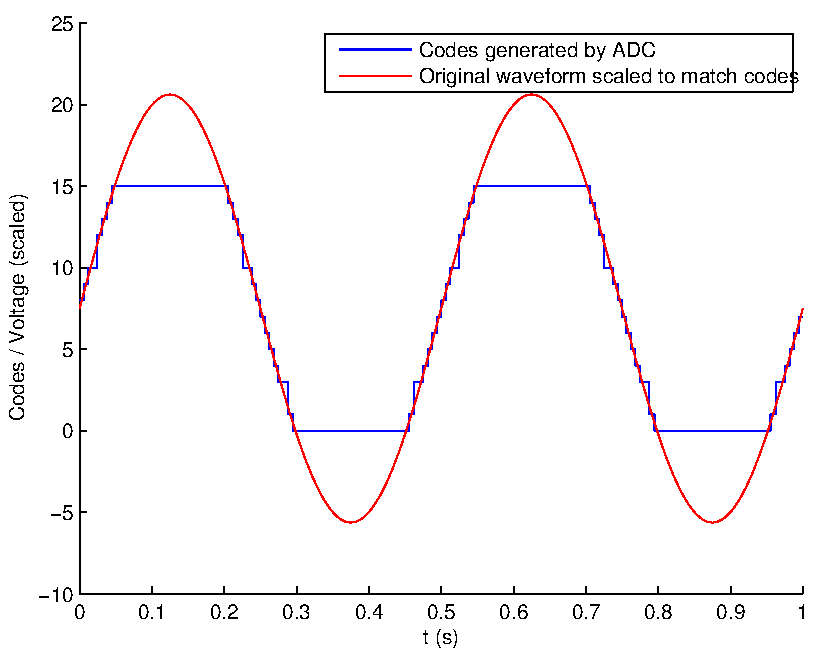
\includegraphics[width=0.7\textwidth]{alg_examples_published/INL-DNL_alg_example_01.pdf}
\end{center}


\subsubsection*{Call algorithm}

\begin{par}
Apply INL algorithm to the input data \lstinline{DI}.
\end{par} \vspace{1em}
\begin{lstlisting}[style=mcode]
DO = qwtb('INL-DNL', DI);
\end{lstlisting}

        \begin{lstlisting}[style=output]
QWTB: no uncertainty calculation
\end{lstlisting} \color{black}
    \begin{par}
Plot results of integral non-linearity. One can clearly observe defects on codes 3 and 11.
\end{par} \vspace{1em}
\begin{lstlisting}[style=mcode]
figure
plot(DO.INL.v, '-x');
xlabel('Transition levels')
ylabel('INL (k)')
% Plot results of differential non-linearity. One can clearly observe defects on transitions 2-3 and
% 10-11.
figure
plot(DO.DNL.v, '-x');
xlabel('Code bins')
ylabel('DNL (k)')
\end{lstlisting}

\begin{center}
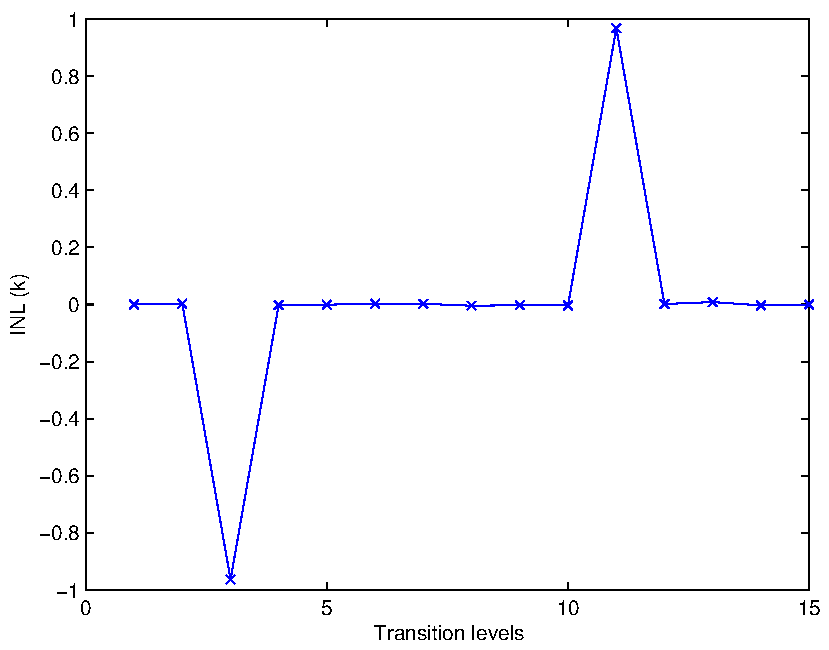
\includegraphics[width=0.7\textwidth]{alg_examples_published/INL-DNL_alg_example_02.pdf}
\end{center}

\begin{center}
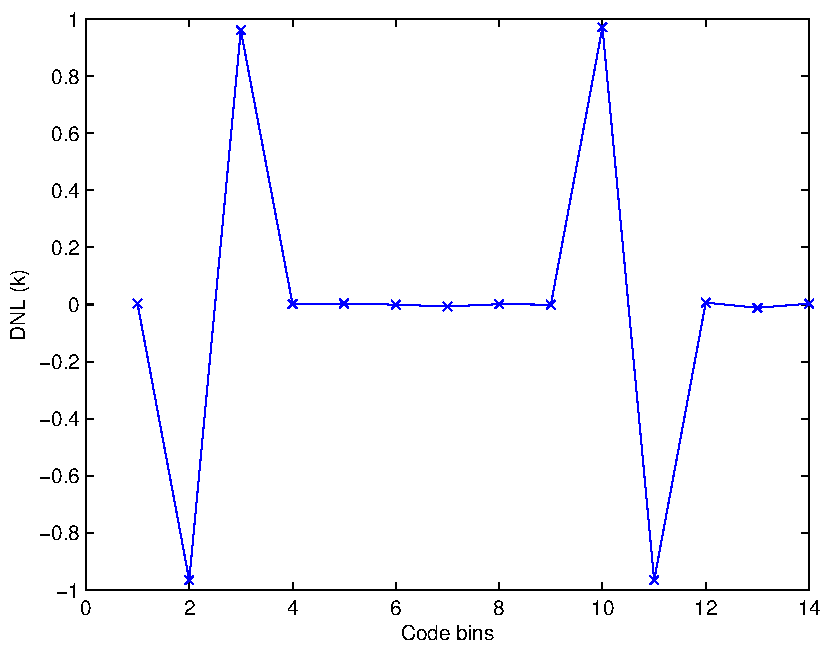
\includegraphics[width=0.7\textwidth]{alg_examples_published/INL-DNL_alg_example_03.pdf}
\end{center}



%%% \end{document}
    
